\chapter{Implementation}

\begin{comment}
Chapter 4: Implementation
The implementation details should be confined to the important, difficult or interesting aspects. Large chunks of code should be avoided, and diagrams and tables should be used to present details clearly.
\end{comment}

\plan{Limited to programming languages only}

\begin{comment}
Statement Management 
Upload
NamedEntityResolution
Suggestions ........................ 19

Prediction
MarkovChain
WeightedArithmeticMean
FiveModelSystem
Confidence

Security Considerations
AccountHijacking
PasswordSecurity
Database Security
Other
\end{comment}

This section is focused on particularly interesting or troublesome parts of implementing the design outlined in \ref{cha:design} and any usage of external libraries. As it was decided the project would be a web application\todo{Should probably mention this in design} the user interface was written in HTML \& CSS, with the interactive elements such as the graphs in JavaScript. PHP was chosen as the server side language used to process the user and the database was implemented using MySQL.

PHP was selected as the server side language because the author had extensive experience in the language, it's original intended use was web development and it is well supported. It's intention of web development means it's well coupled with HTML and provides many libraries to handle it, giving the language a significant advantage over languages such as Python and Java which can be adapted for web use. A key disadvantage of PHP is that is it weak typed which lead to some issues during development where objects of the wrong type were passed into functions. This disadvantage was considered and it was decided the advantages outweighed the disadvantages.

The project uses a PHP Framework, written by the author \todo{This doesn't make sense} called pegFramework. Using a framework has several key advantages over writing the whole system.

Frameworks:
Provide standardised code and file organisation - pegFramework has a well defined code structure, code is organised in a predefined way and split into modules
MVC - Model View Controller - using the MVC pattern with a framework ensures models (data structures), views (page contnet) and controllers are separate, improving cohesiveness and decreasing coupling.
Utilities and libraries - frameworks handle all the standard web design code, including routing, security, controllers, rendering the template and caching.

MySQL was selected as the database language because it's well supported by PHP and because it provides Natural Language Searching out of the box, which supports free-text queries and can calculate the relevance of a record in the database to a search term. This is used to power the suggestions section of the website and for user entered searches.

Server Side Libraries:

Twig - a template engine that takes collections of PHP objects and following a provided .html template build the output sent to the browser. In addition it provides caching of the generated templates and output, leading to significant speed increases for the end user.

Propel - an object relational mapping (ORM) library for PHP. Propel takes a database schema defined in XML and generates PHP objects that represent the schema which can be saved to and loaded from the database.

Less - CSS pre-processor that extends CSS, adding additional features and inheritance. `.less` files compile to `.css`

Front End

Bootstrap - framework for CSS development that provides grid and stuff

jQuery - javascript development framework that abstracts differences in browser behaviour and provides shorthands to common tasks such as ajax requests

Pines Nofity - alerts

Chosen - javascript libray to make dropdown boxes better

Highcharts - charting library for the UI

\section{Statement Management}

\subsection{Upload}
OFX is an XML like format called SGML. PHP has inbuilt libraries for parsing XML called SimpleXML simplexml\_load\_string loads an XML file from a string. To parse the OFX, PHP attempts to parse it as an XML file and captures any exceptions. If exeptions are found it attempts to convert the SGML XML so it can be pased by PHP as per 

%http://stackoverflow.com/questions/15735330/how-to-parse-a-ofx-version-1-0-2-file-in-php and http://www.hanselman.com/blog/PostprocessingAutoClosedSGMLTagsWithTheSGMLReader.aspx

\todo{Comparison of SGML and XML}

For each line of the SGML it trims whitespace including (x,y,z), converts the charset ot UTF-8 so it's valid in PHP and if no closing tag is found, appends a closing tag

\lstset{style=phpcolor}
\begin{lstlisting}
foreach(preg_split("/((\r?\n)|(\r\n?))/", $this->OFXContent) as $line){
        		
        	// Trim whitespace
        	$line = trim($line);
        	if ($line === '') continue;
        
        	// Convert charset to UTF-8
        	$line = iconv($charset, 'UTF-8', $line);
        	if (substr($line, -1, 1) !== '>') {
        		list($tag) = explode('>', $line, 2);
        		$line .= '</' . substr($tag, 1) . '>';
        	}
        	$buffer .= $line ."\n";
}
\end{lstlisting}

Having parsed the SGML into objects it can just be navigated following the specification and converted to arrays of information for each transaction, refered to as movements. These movements look like XYZ; and can then be convered into the Transaction objects most of the fields are handled automatically but dates need to be handled specifically.

QIF is handled in a different manor as there are no native libraries to parse it's format. As per the Fig. \ref{fig:qifofxformat} shown in section \ref{subsection:upload} shown in  the format is a list of individual movements, with each terminated a \^. Each field associated with an individual movement is identified with a letter, explaining the contents of that line.
% 
The field types that the project was interested in and parses are shown in Table \ref{table:qiffields}.

\begin{table}[h]
\begin{tabular}{ll}
D                  & Date           \\
T                  & Amount         \\
C                  & Cleared status \\
P                  & Payee          \\
M                  & Memo           \\
\textasciicircum   & End of entry  
\end{tabular}
\caption{QIF fields parsed by the project}
\label{table:qiffields}
\end{table}

In a similar manor to parsing the OFX files, the application loops though all the lines found in the file, switching on the identifier and sorting the information into an array representing that movement. 

\lstset{style=phpcolor}
\begin{lstlisting}[float,floatplacement=H]

// QIF line identifier
$id = substr($line, 0, 1);

// Rest of the line
$content = trim(substr($line, 1, strlen($line)));

switch ($id) {
	// End of entry
	case '^':
		// Completed transaction append to our list and reset
		$this->movements[] = $newMovement;
		$newMovement = array();
		break;
		
	// Amount
	case 'T':
		$newMovement["value"] = floatval(preg_replace("/[^0-9.-]/", "", $content));
		break;
		
	// Date
	case 'D':
		$newMovement["date"] = $content;
		break;
		
	// etc ...
\end{lstlisting}

As outlined in section \ref{subsection:upload} the conversion from the array to a Transaction object is slightly more involved due to unknown date format. To implement this in PHP, before begining the conversion, all movements are tested against two regular expressions (regex), representing the possible formats of the dates, which are visualised as graphs in Fig. \ref{fig:regex-dmy} and \ref{fig:regex-mdy}. 

\lstset{style=phpcolor}
\begin{lstlisting}[float,floatplacement=H]
$dmy = true;
$mdy = true;
foreach($this->getMovements() as $movement)
	if(!preg_match('#(0[1-9]|[12][0-9]|3[01])[-/](0[1-9]|1[012])[-/](19|20|21)?\d\d#', $date))
		$dmy = false;
	
	if(!preg_match('#(0[1-9]|1[012])[-/](0[1-9]|[12][0-9]|3[01])[-/](19|20|21)?\d\d#', $date))
		$mdy = false;
\end{lstlisting}

\begin{figure}[h]
    \centering
    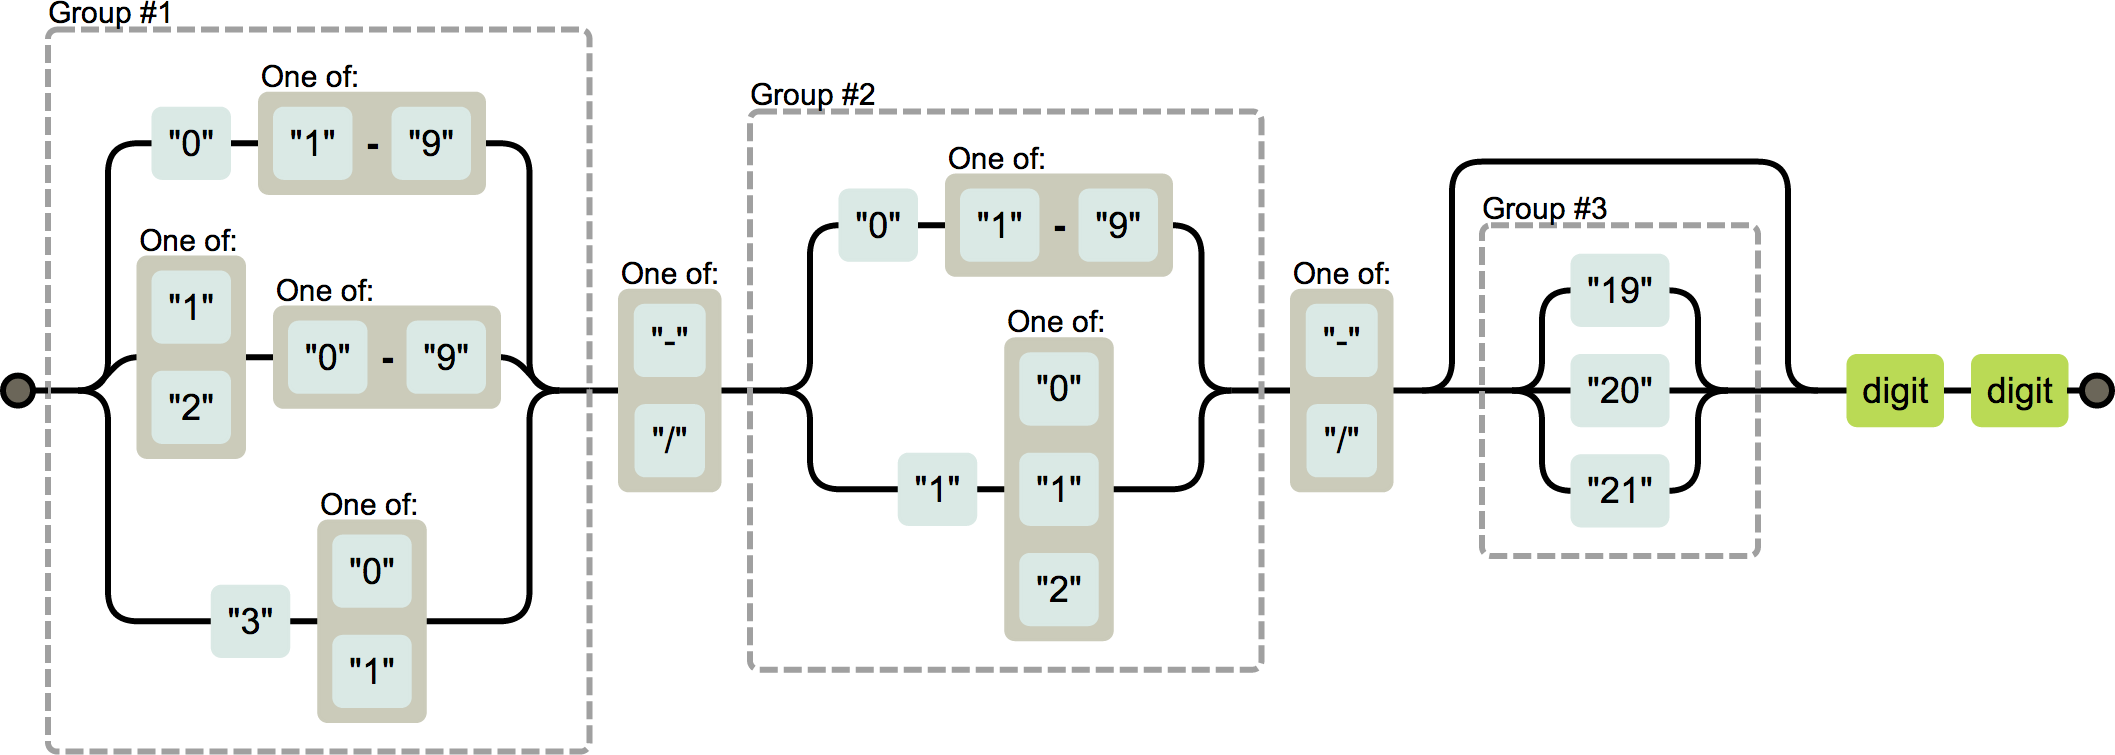
\includegraphics[width=\textwidth]{implementation/regex-dmy}
    \caption[Regular expression used to match d-m-Y]{Railroad diagram of the regex used to match format d-m-Y}
    \label{fig:regex-dmy}
\end{figure}

\begin{figure}[h]
    \centering
    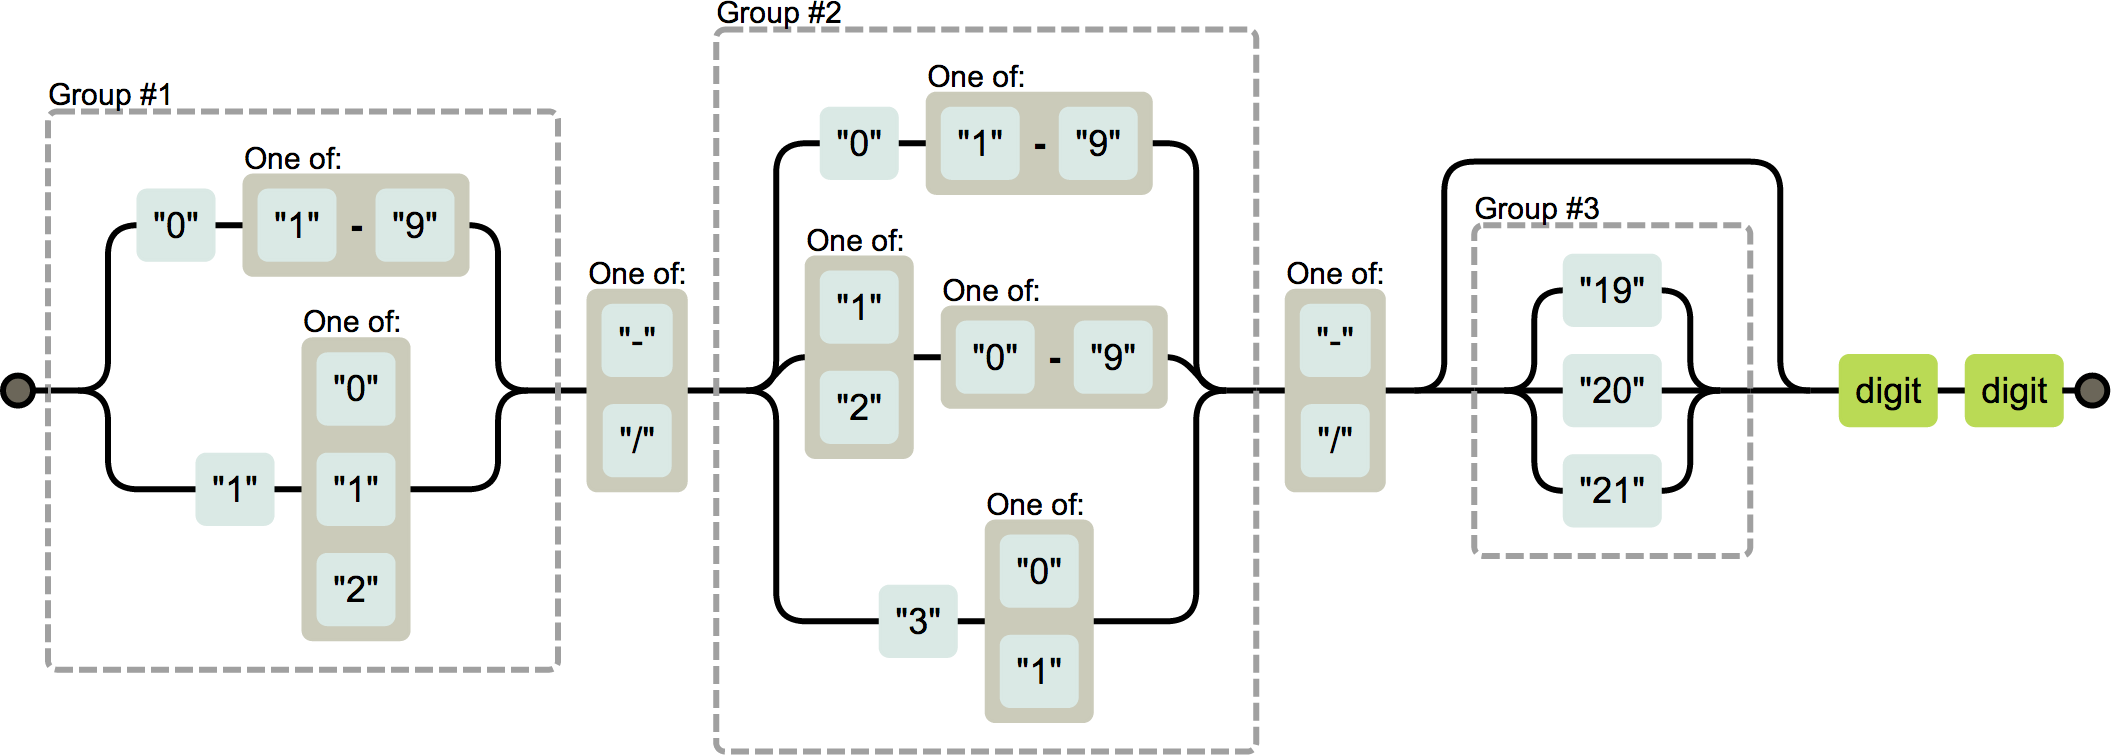
\includegraphics[width=\textwidth]{implementation/regex-mdy}
    \caption[Regular expression used to match m-d-Y]{Railroad diagram of the regex used to match format m-d-Y}
    \label{fig:regex-mdy}
\end{figure}

Having considered all the movements found in the file, the application has either decided on one of the date formats or prompts the user to decide the appropriate format, as seen in Fig. \ref{fig:dateformat-prompt}.

\lstset{style=phpcolor}
\begin{lstlisting}[float,floatplacement=H]
if($dmy && $mdy || !$dmy && !$mdy)
    // ... prompt the user
else
    // ... continue the conversion using the detected month format
\end{lstlisting}

\begin{figure}[h]
    \centering
    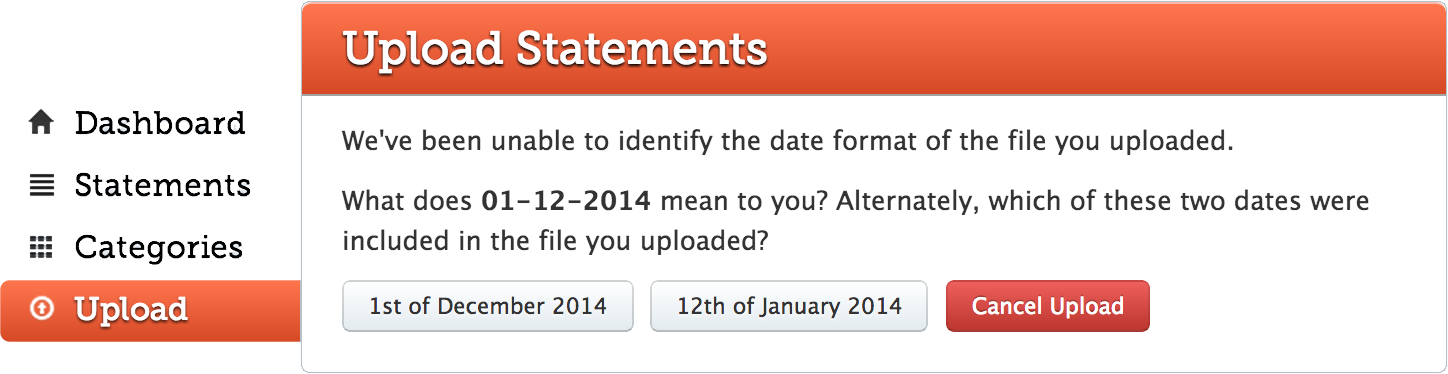
\includegraphics[width=0.70\textwidth]{implementation/dateformat-prompt}
    \caption{UI Prompt when the application is unable to decide an upload's date format}
    \label{fig:dateformat-prompt}
\end{figure}

\subsection{Named Entity Resolution}
The implemented the mapping architecture outlined in the design, the majority of the named entity resolution is done in the \lstinline{setTransactor} method of the Transaction object, which is called when setting the name of transactor for a each transaction found in the uploaded file.   
% 
The method performs three key actions, tidying the string, removing common notation added by banking institutions and checking the database for known user and global transactors, otherwise creating a new one.
% 
To avoid unnecessary duplication in the mappings table the \gls{transactor} names are normalised before checking for an existing name, this normalisation was added to combat the various different ways which banks store the transactor names which were discovered during testing. The modifications included: padding with spaces, replacing spaces with underscores/tabs, or including non alphanumeric letters; some examples are shown in Table \ref{table:cleaningstrings}.
%
Having normalised the input, the next step was to remove any numeric identifiers which had been added and move that detail to another field. Examples of such identifiers included store id's for shops with multiple outlets and account numbers for transfers between accounts, if this detail wasn't removed a separate mapping would be created for transactions referencing the same entity, leading to unnecessary duplication. The identifiers were removed using a regex, expressed in Fig. \ref{fig:regex-transactor} which only captures numbers found at the end of the string requiring at least two digits, these additional constraints were added to preserve \glspl{transactor} with numbers in their name, such as \inlinetext$H3G$ and \inlinetext$SUPERMERCADO 3$.
%
The final step checks for existing \glslink{globaltransactor}{GlobalMapping} or \glslink{usertransactor}{UserMapping} objects in the database and if found associates that mapping with this transaction. If neither mapping's are found a new \glslink{usertransactor}{UserMapping} object is created, persisted and associated with the transaction. Differing from the original plan, fuzzy matching\footnote{ Finding strings that approximately rather than exactly match} of the transactor name when searching for existing transactors is not performed as this functionality was moved to the suggestion wizard.
%
The full code for the `setTransactor` method is shown in Fig. \ref{fig:settransactor}.

\lstset{language=textwithspaces,style=showspaces}
\begin{table}[h]
\centering
\begin{tabular}{ll}
Raw Transactor Name & Occurrences \\
\inlinetext$TESCO STORES 5128$   & 87         \\
\inlinetext$TESCO STORES 2977$   & 68         \\
\inlinetext$TESCO_STORES$        & 14         \\
\inlinetext$SACAT MARKS    AND$  & 33         \\
\inlinetext$SACAT MARKS  AND$    & 16         \\
\inlinetext$WILKINSON $          & 22         \\
\inlinetext$WILKINSON$           & 8          \\        
\inlinetext$TO A/C 00000000$\footnote{Account number removed} & 2  
\end{tabular}
\caption{Examples of the raw transactor names found on uploaded statements}
\label{table:cleaningstrings}
\end{table}

\begin{figure}[h]
    \centering
    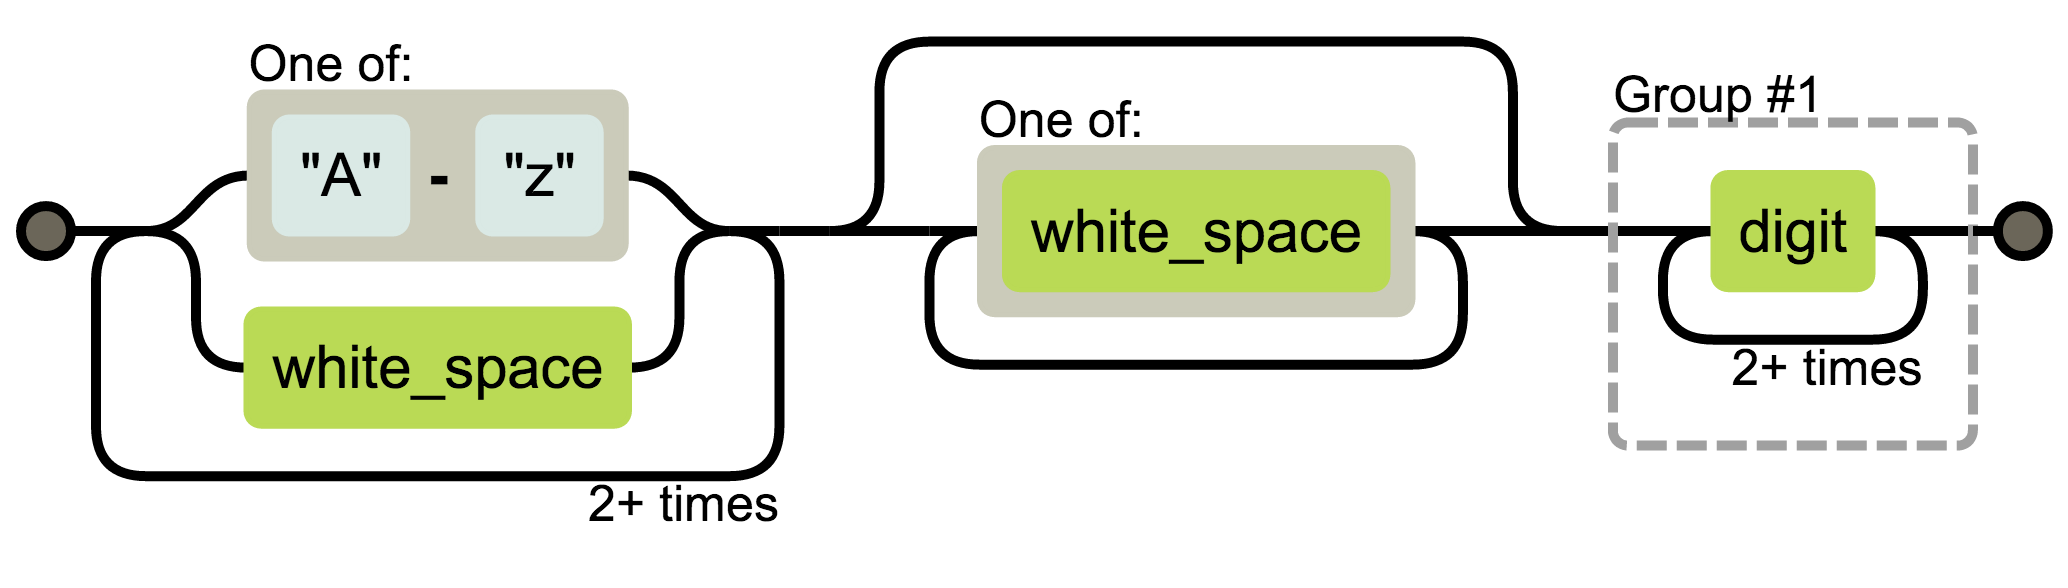
\includegraphics[width=\textwidth]{implementation/regex-transactor}
    \caption[Regular expression used to match the transactor name]{Railroad diagram of the regex used to tidy the transactor name}
    \label{fig:regex-transactor}
\end{figure}

\subsection{Suggestion Wizard}
The suggestion wizard (Fig \ref{fig:suggestion-wizard}) was added to the project in response to observations during lab usability testing. Originally the suggestions were only found on each unmapped transactors page (Fig. \ref{fig:view-reference-suggestions}) to speed up the process of mapping a reference to an existing transactor.  Users appeared to spend a lot of time manually categorising each individual transactor by searching their statement for an unknown transactor, opening that transactors details and then filling in the appropriate forms or clicking on a suggestion, following an activity diagram similar to Fig. \ref{fig:transactor-mapping-activity}.

\begin{figure}[h]
    \centering
    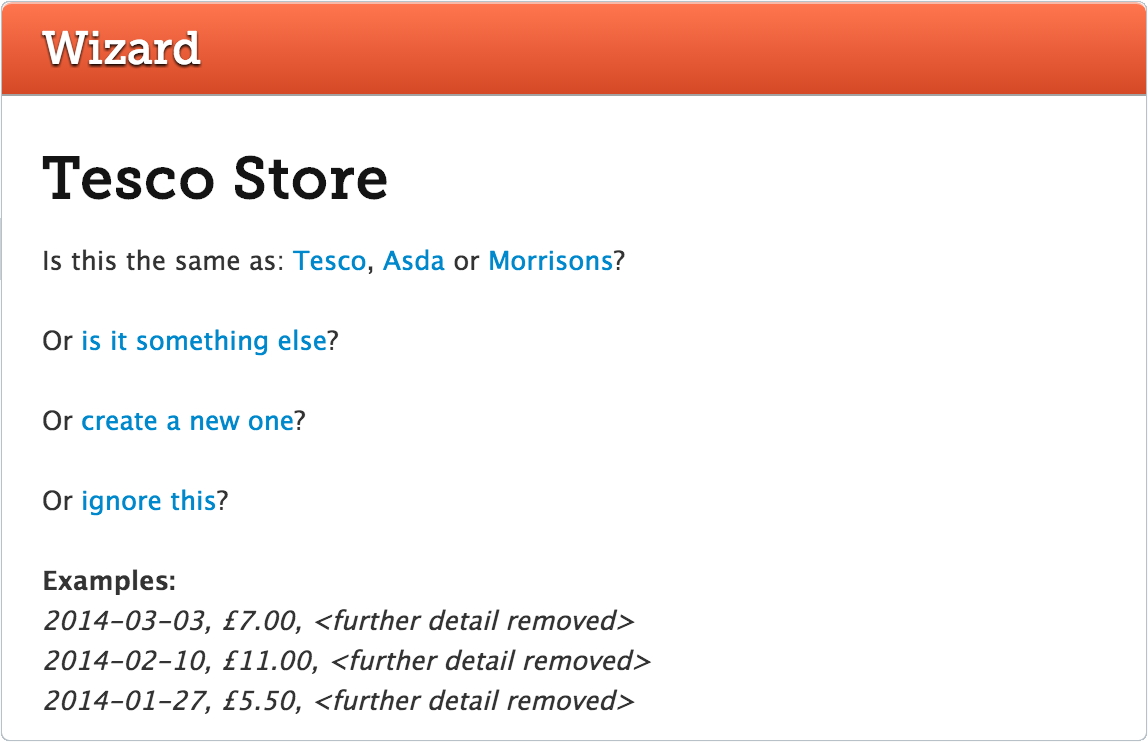
\includegraphics[width=\textwidth]{implementation/suggestion-wizard}
    \caption[Suggestion wizard UI]{Suggestion wizard UI\protect\footnotemark}
    \label{fig:suggestion-wizard}
\end{figure}
\footnotetext{Potentially personally identifiable information removed}

\begin{figure}[h]
    \centering
    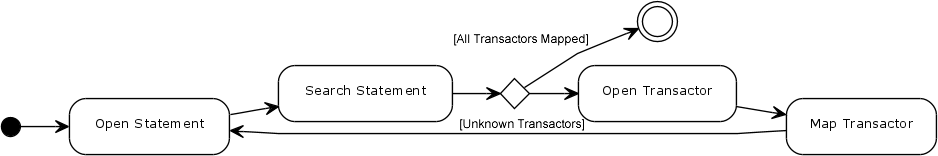
\includegraphics[width=\textwidth]{implementation/transactor-mapping-activity}
    \caption{Activity diagram for mapping individual transactors}
    \label{fig:transactor-mapping-activity}
    
    \begin{comment}
(start)->(Open Statement)->(Search Statement)-><a>->(end)
<a>->(Open Transactor)->(Map Transactor)->(Open Statement)
    \end{comment}
\end{figure}

\begin{figure}[h]
    \centering
    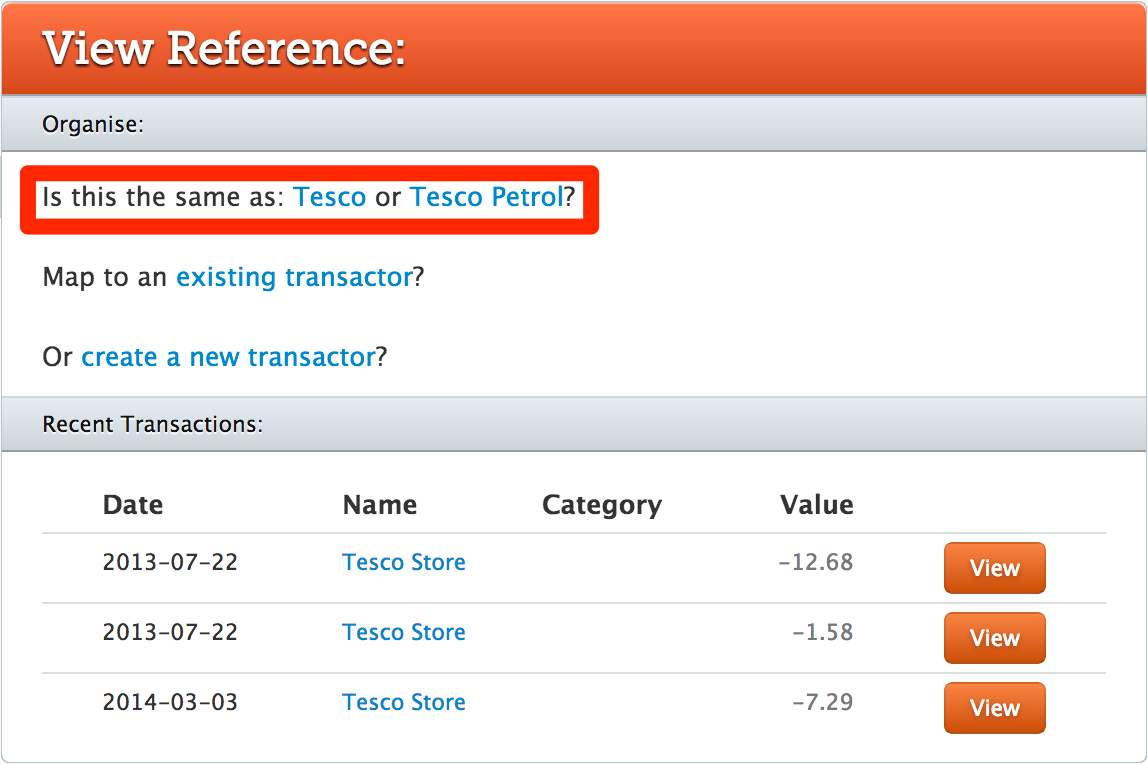
\includegraphics[width=\textwidth]{implementation/view-reference-suggestions}
    \caption{Suggestions shown on the Transactor (reference) page}
    \label{fig:view-reference-suggestions}
\end{figure}

The wizard was designed to streamline and speed up this process as well as making it easier for the user to follow. Each unmapped transactor is displayed in turn, starting with the one with the most transactions (encouraging the user to map the ones they shop at more often first). On each step, the user can; follow the suggestions, manually map the reference to an existing transactor, create a new transactor or ignore the reference for now. A step-by-step view of this process is shown in section \ref{subsection:suggestion-wizard-walkthrough}.

During the process feedback is displayed to the user using notifications that appear over the wizard and are coloured according to validation style convention, with red warning of an error and green confirming success (Fig. \ref{fig:suggestion-notification}). 

\begin{figure}[h]
    \centering
    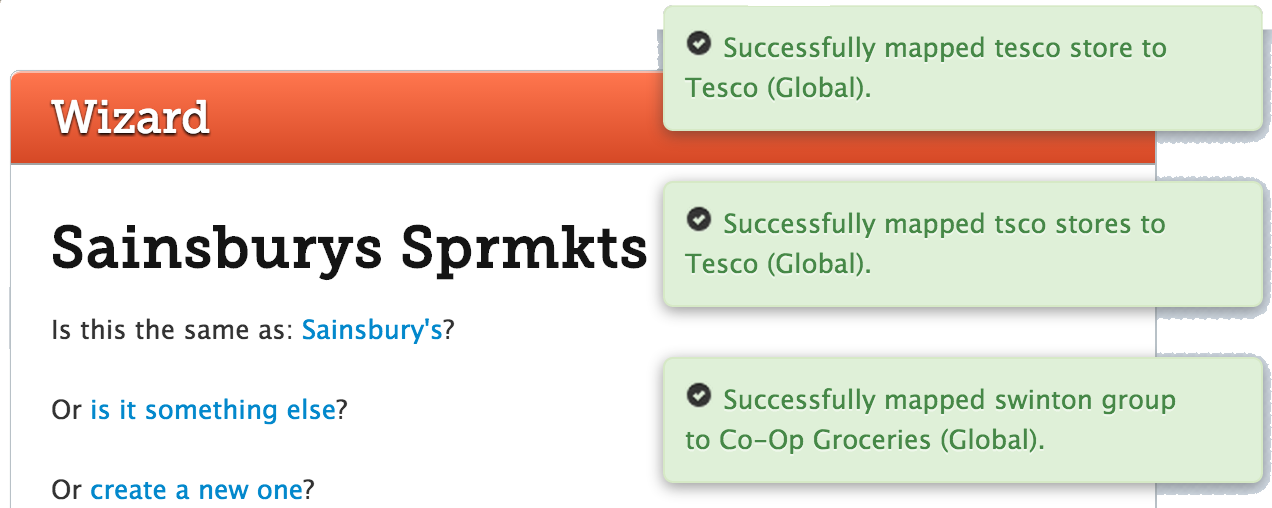
\includegraphics[width=\textwidth]{implementation/suggestion-notification}
    \caption{Notifications shown during the suggestion wizard}
    \label{fig:suggestion-notification}
\end{figure}

By following the wizard users are able to quickly map the majority of their transactions in an easy to follow way, as can be shown by the activity diagram in Fig. \ref{fig:suggestion-wizard-activity}.

\begin{figure}[h]
    \centering
    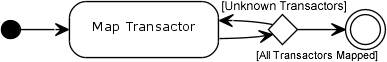
\includegraphics[width=0.6\textwidth]{implementation/suggestion-wizard-activity}
    \caption{Activity diagram for mapping transactors using the suggestion wizard}
    \label{fig:suggestion-wizard-activity}
    
    \begin{comment}
(start)->(Map Transactor)-><a>->(end)
<a>->(Map Transactor)
    \end{comment}
\end{figure}

The wizard itself is powered by Ajax\footnote{Asynchronous JavaScript and XML}, which sends requests to a backend RESTful API which proves access to the unmapped transactors found for the user. The requests and responses are sent as JSON\footnote{JavaScript Object Notation} which is supported natively by both PHP and JavaScript. A GET request to \lstinline{/ajax/transactor/suggestions} returns a collection of unmapped transactors including associated examples which are then added to the UI using JavaScript.
%
Mapping (including following a suggestion) and creating a new transactor are both handled by POST requests to the same API. Mapping sends a request to \lstinline{/ajax/transactor/map} containing the ID of the user mapping and global mapping  and creation sends a request to \lstinline{/ajax/transactor/create} including the user mapping ID to associate with the new transactor. 
%
Examples of the JSON communication are shown in Fig. \ref{fig:json-examples}.

On the backend, all JSON serialisation is handled by implementing the \inlinephp{JsonSerializable} interface on all objects that need to be JSON encoded. This allows the native function \inlinephp{json_encode(\$object)} to correctly encode the object into JSON using the data returned by the abstract method `jsonSerialize` defined in the interface. The final inheritance diagram for the mapping, transactor and transaction objects is shown in Fig. \ref{fig:mapping-inheritance-diagram}.

\begin{figure}[h]
    \centering
    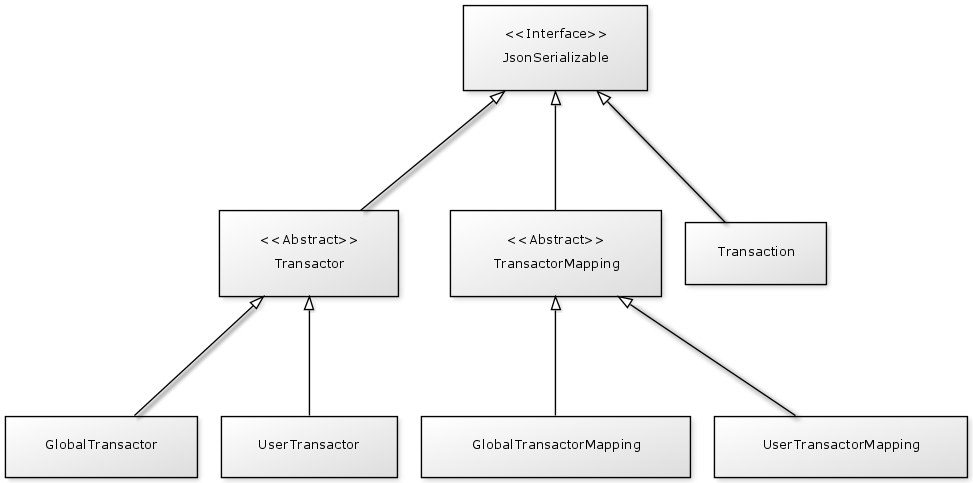
\includegraphics[width=\textwidth]{implementation/json-serializable}
    \caption{Inheritance diagram of JsonSerializable objects}
    \label{fig:mapping-inheritance-diagram}
    
    \begin{comment}
[<<Interface>> JsonSerializable]^-[<<Abstract>> Transactor]
[<<Interface>> JsonSerializable]^-[<<Abstract>> TransactorMapping]
[<<Interface>> JsonSerializable]^-[Transaction]
[<<Abstract>> TransactorMapping]^-[UserTransactorMapping]
[<<Abstract>> TransactorMapping]^-[GlobalTransactorMapping]
[<<Abstract>> Transactor]^-[UserTransactor]
[<<Abstract>> Transactor]^-[GlobalTransactor]
    \end{comment}
\end{figure}

The suggestions themselves are made by searching for known global mappings, user mappings, global transactors and user transactors\footnote{In the order of preference} that are similar to the reference name a suggestion is being made for. This is done using the Natural Language Full-Text Search functions provided by MySQL. These functions, including \inlinesql$MATCH$, use a Vector Space Model to rank the relevance of a field relative to the input and signify this relevance using a decimal number, which means it can be treated as a standard field by the database and used to order the results.  \parencite{mysql2014searches}. 

When searching for suggestions the application finds the five most relevant mappings or transactors, according to full text search, loads those objects from the database using the ORM. As the ORM tool uses doesn't have support for full text search a raw SQL query was written that uses PDO's\footnote{PHP Data Objects extension for accessing databases} prepared statements functionality to send the parameters to the database server, avoiding SQL injection. The query for finding global transactor mappings as part of the \inlinephp{GetCloseTransactorMappings} method in the GlobalTransactorMappingPeer class is shown in Fig. \ref{fig:sql-match-query}, where \inlinesql{:identifier} is replaced by the server with the passed parameters.

\begin{figure}
\centering
\begin{lstinline}[language=sql]
SELECT *, MATCH(:nameColumn) AGAINST (:name) AS 'score'
FROM :tableName
	WHERE :transactorID IS NOT NULL
	HAVING `score` > :minScore OR :nameColumn = :name
ORDER BY `score` DESC
LIMIT 5
\end{lstinline}
\caption{SQL Query for selecting similar mappings or transactors using PDO}
\label{fig:sql-match-query}
\end{figure}

\section{Prediction}
The key difficulty of implementing the prediction functionality was designing a data structure that allowed predictions to be read by column or by row in order to generate the table output shown in Fig. \ref{}. Ordinarily a multidimensional array or a dictionary of dictionaries would be used, however in this case it must be possible to access the data by subcategory as well as by month or date

\subsection{Markov Chain Models}
\plan{Use of MySQL to find similar, how that works, alternatives}

\subsection{Weighted Arithmetic Mean}
\label{section:suggestion-implementation}
\plan{How it uses the above, how the whole user/global thing works}

\subsection{Five Model System}
\plan{Why I chose first order markov chains, alternatives to that etc...}

\section{Security Considerations}
\plan{How does that work, why is it good?}

\subsection{Hijacking}
\plan{How was is a model chosen for the user?}

\subsection{Password Security}
\plan{How was is a model chosen for the user?}

\subsection{Hijacking}
\plan{Database storage}


